\newpage \section{Results}
\label{sec:results}

The stability of CMS integrated luminosity for Phase I pixel detector calculated using PCC method is investigated using late Run2018D veto list.

\begin{figure}[H]
  \centering
  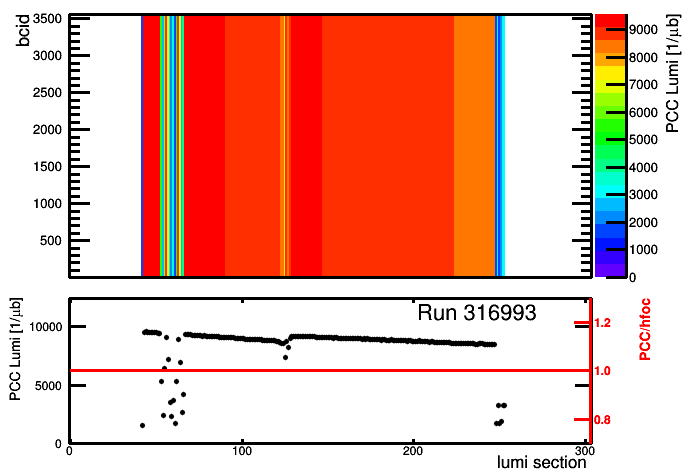
\includegraphics[width=0.52\columnwidth]{./316993.png}
  \caption{Top: Bunch crossing id (bcid) and PCC luminosity as a function of lumi section (1 lumi section is 23.36s). Bottom: PCC lumi as a function of lumi section using late run 2018D veto list for Run2018A.}
  \label{fig:CMS}
\end{figure}


\begin{figure}[H]
  \centering
  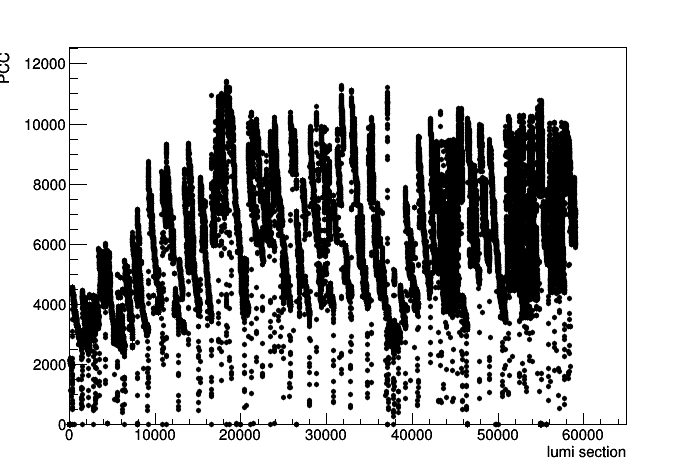
\includegraphics[width=0.52\columnwidth]{./ls_lumi.png}
  \caption{PCC luminosity ($\mu b^{-1}$) as a function of luminosity section (1 lumi section is 23.36s) for Run2018A.}
  \label{fig:CMS}
\end{figure}


\begin{figure}[H]
  \centering
  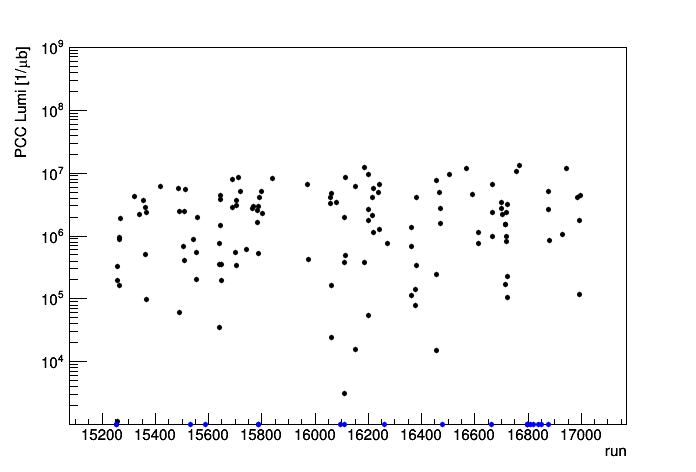
\includegraphics[width=0.52\columnwidth]{./runs.png}
  \caption{PCC luminosity ($\mu b^{-1}$) as a function of run number for Run2018A.}
  \label{fig:CMS}
\end{figure}


\begin{figure}[H]
  \centering
  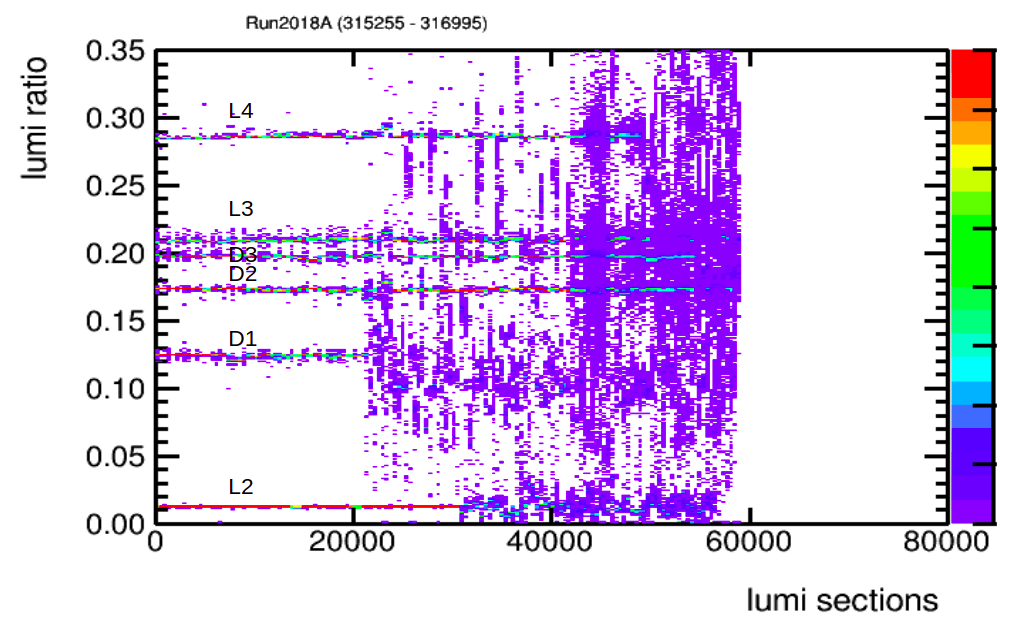
\includegraphics[width=0.52\columnwidth]{./2018A_lumiratio.png}
  \caption{Luminosity ratios for various subdetectors L2, L3, L4, D1, D2, D3 of pixel detector as a function of lumi section for Run2018A.}
  \label{fig:CMS}
\end{figure}



\begin{figure}[H]
  \centering
  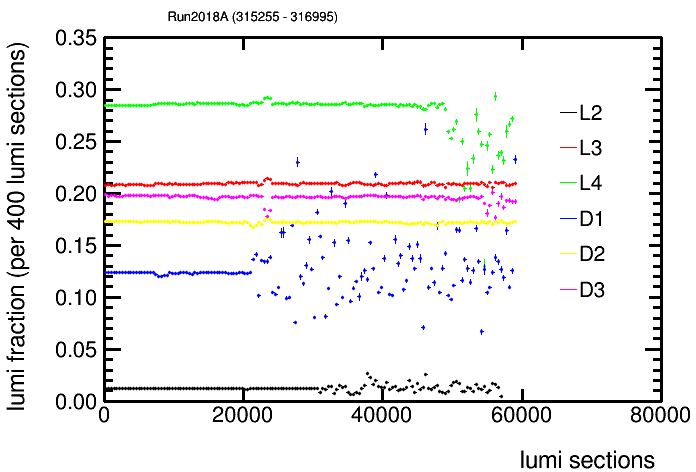
\includegraphics[width=0.52\columnwidth]{./ProfileXcombined_new.png}
  \caption{X Profile of luminosity ratios vs lumi section graph for various subdetectors L2, L3, L4, D1, D2, D3 of pixel detector showing luminosity fraction as a function of lumi section (1 lumi section is 23.36s) for Run2018A.}
  \label{fig:CMS}
\end{figure}





\begin{figure}[H]
  \centering
  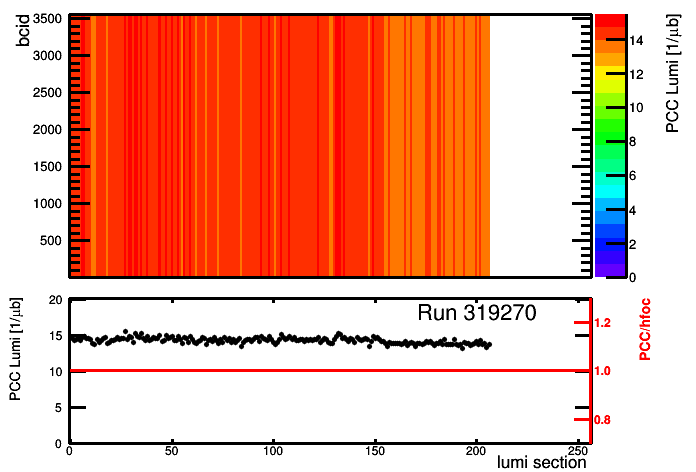
\includegraphics[width=0.52\columnwidth]{./319270.png}
  \caption{Top: Bunch crossing id (bcid) and PCC luminosity as a function of lumi section. Bottom: PCC lumi as a function of lumi section using late run 2018D veto list for Run2018B.}
  \label{fig:CMS}
\end{figure}


\begin{figure}[H]
  \centering
  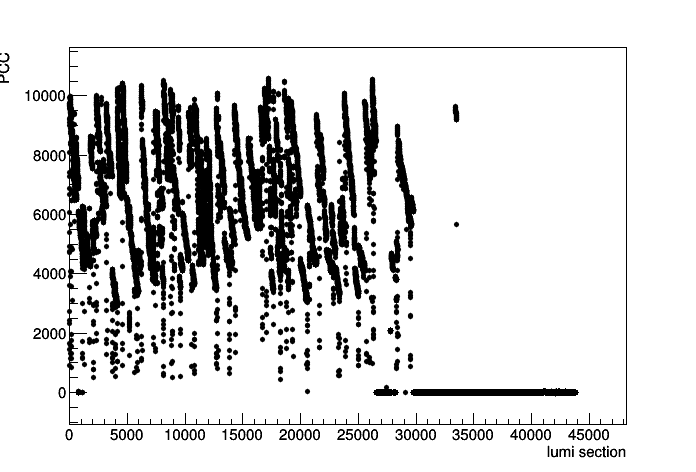
\includegraphics[width=0.52\columnwidth]{./ls_lumi_2018B.png}
  \caption{PCC luminosity as a function of lumi section for Run2018B.}
  \label{fig:CMS}
\end{figure}


\begin{figure}[H]
  \centering
  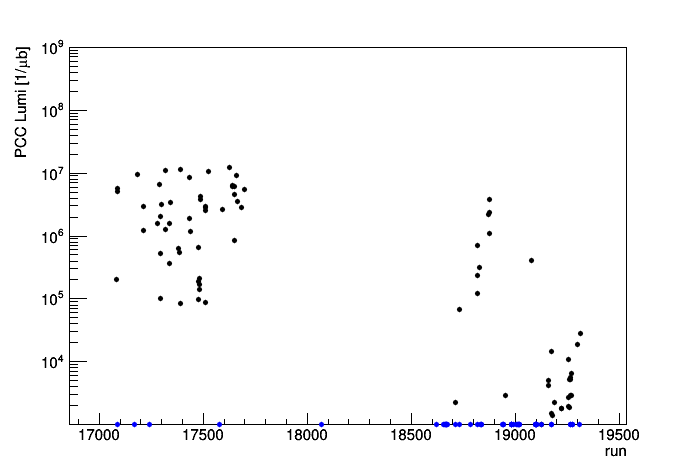
\includegraphics[width=0.52\columnwidth]{./runs_2018B.png}
  \caption{PCC luminosity as a function of run number for Run2018B.}
  \label{fig:CMS}
\end{figure}


\begin{figure}[H]
  \centering
  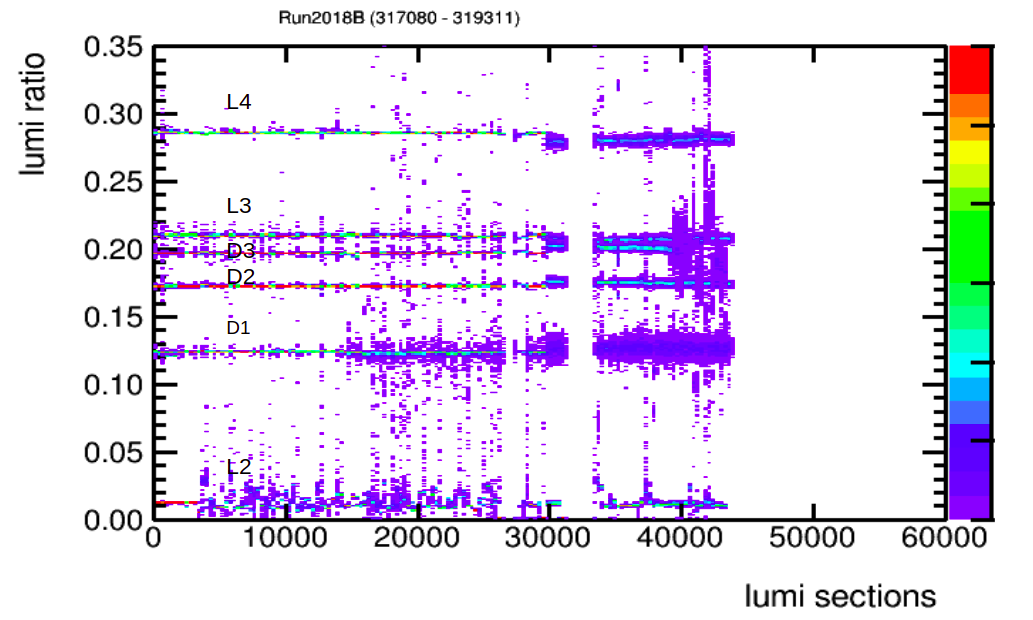
\includegraphics[width=0.52\columnwidth]{./2018B_lumiratio.png}
  \caption{Luminosity ratios for various subdetectors L2, L3, L4, D1, D2, D3 of pixel detector as a function of lumi section for Run2018B.}
  \label{fig:CMS}
\end{figure}



\begin{figure}[H]
  \centering
  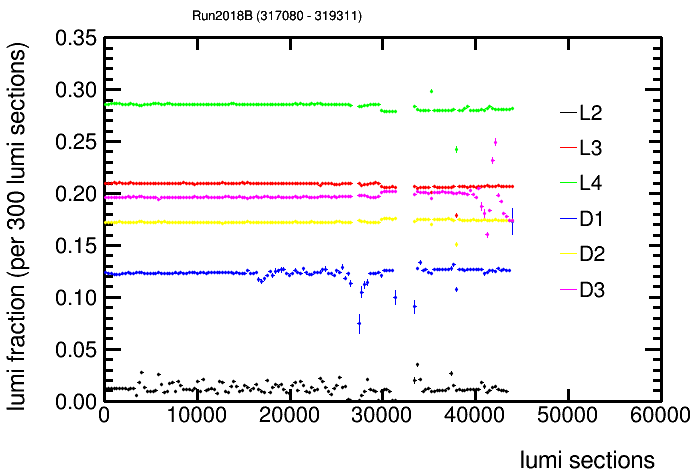
\includegraphics[width=0.5\columnwidth]{./ProfileXcombinedB_new.png}
  \caption{X Profile of luminosity ratios vs lumi section graph for various subdetectors L2, L3, L4, D1, D2, D3 of pixel detector showing luminosity fraction as a function of lumi section for Run2018B.}
  \label{fig:CMS}
\end{figure}



\begin{figure}[H]
  \centering
  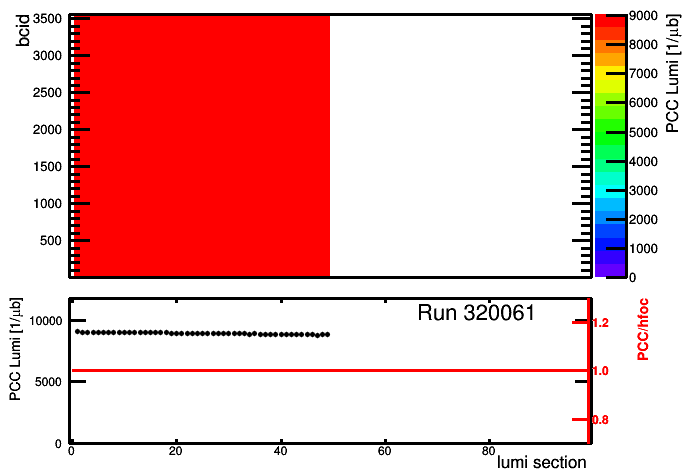
\includegraphics[width=0.5\columnwidth]{./320061.png}
  \caption{Top: Bunch crossing id (bcid) and PCC luminosity as a function of lumi section. Bottom: PCC lumi as a function of lumi section using late run 2018D veto list for Run2018C.}
  \label{fig:CMS}
\end{figure}


\begin{figure}[H]
  \centering
  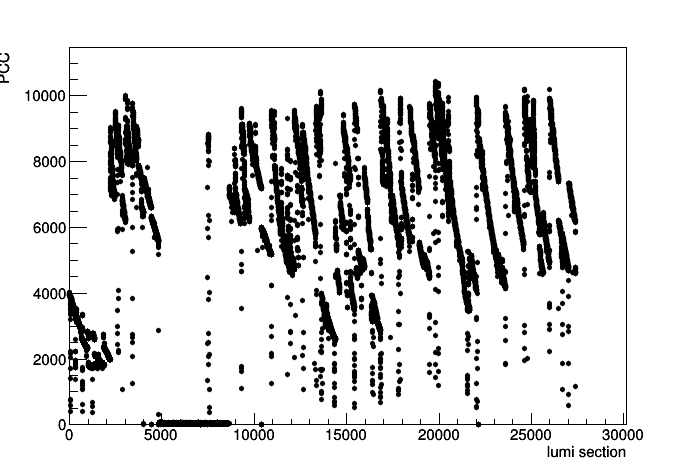
\includegraphics[width=0.5\columnwidth]{./ls_lumi_2018C.png}
  \caption{PCC luminosity as a function of lumi section for Run2018C.}
  \label{fig:CMS}
\end{figure}


\begin{figure}[H]
  \centering
  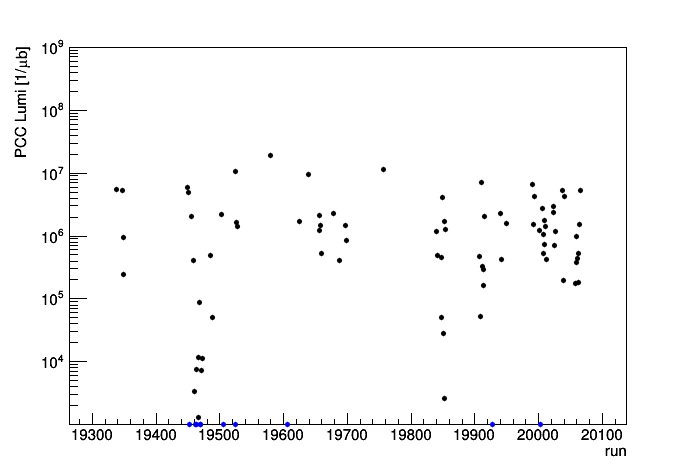
\includegraphics[width=0.5\columnwidth]{./runs_2018C.png}
  \caption{PCC luminosity as a function of run number for Run2018C.}
  \label{fig:CMS}
\end{figure}


\begin{figure}[H]
  \centering
  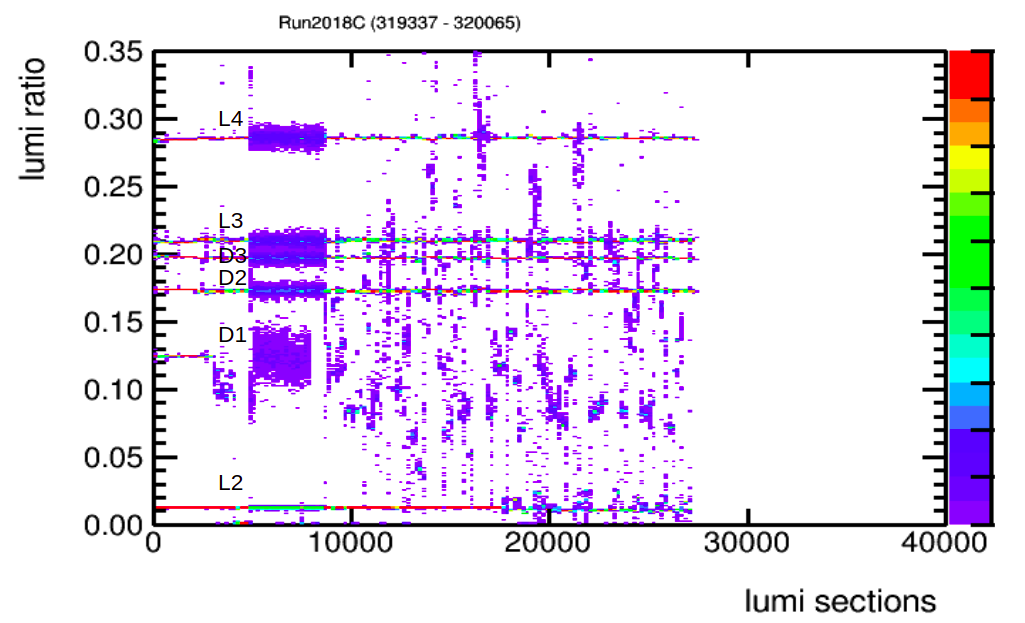
\includegraphics[width=0.5\columnwidth]{./2018C_lumiratio.png}
  \caption{Luminosity ratios for various subdetectors L2, L3, L4, D1, D2, D3 of pixel detector as a function of lumi section for Run2018C.}
  \label{fig:CMS}
\end{figure}


\begin{figure}[H]
  \centering
  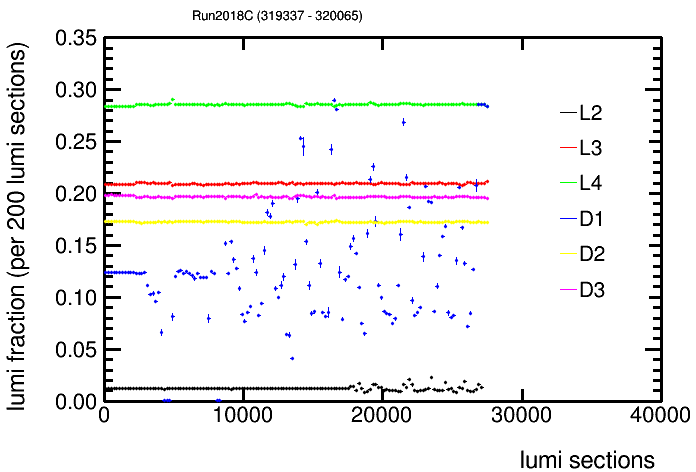
\includegraphics[width=0.5\columnwidth]{./ProfileXcombinedC_new.png}
  \caption{X Profile of luminosity ratios vs lumi section graph for various subdetectors L2, L3, L4, D1, D2, D3 of pixel detector showing luminosity fraction as a function of lumi section for Run2018C. \cite{lumidpg}}
  \label{fig:CMS}
\end{figure}

